
% Sec 4.3.1
\subsection{Equações de Euler para um corpo rígido em órbita circular}
\label{sec_atitude_inercial}

A dinâmica de atitude de uma espaçonave rígida em órbita circular pode ser descrita pelas equações de Euler escritas em relação ao referencial orbital \gls{lvlh}. Nessa formulação, a atitude não é tratada apenas como uma rotação do corpo em relação ao referencial inercial, mas como um movimento angular definido em relação ao sistema orbital, o que permite incorporar explicitamente o acoplamento entre órbita e atitude.

Para essa formulação, adotam-se os seguintes referenciais:
\begin{itemize}
    \item Referencial $N$: referencial inercial;
    \item Referencial $A$: referencial orbital \gls{lvlh}, com origem no \gls{cdm} da espaçonave;
    \item Referencial $B$: referencial fixo ao corpo da espaçonave, cujos eixos coincidem com os eixos principais de inércia.
\end{itemize}

A Figura~\ref{fig_corporigido_wie} apresenta a geometria de um corpo rígido em órbita circular, incluindo o referencial inercial $N$, o referencial orbital $A$, o referencial fixo ao corpo $B$, o vetor posição $\vec{R}_c$ do \gls{cdm} da espaçonave em relação ao centro da Terra, o vetor $\vec{\rho}$ do elemento de massa $dm$ em relação ao \gls{cdm} e o vetor $\vec{R}$ do elemento de massa $dm$ em relação ao centro da Terra.

\begin{figure}[H]
\centering
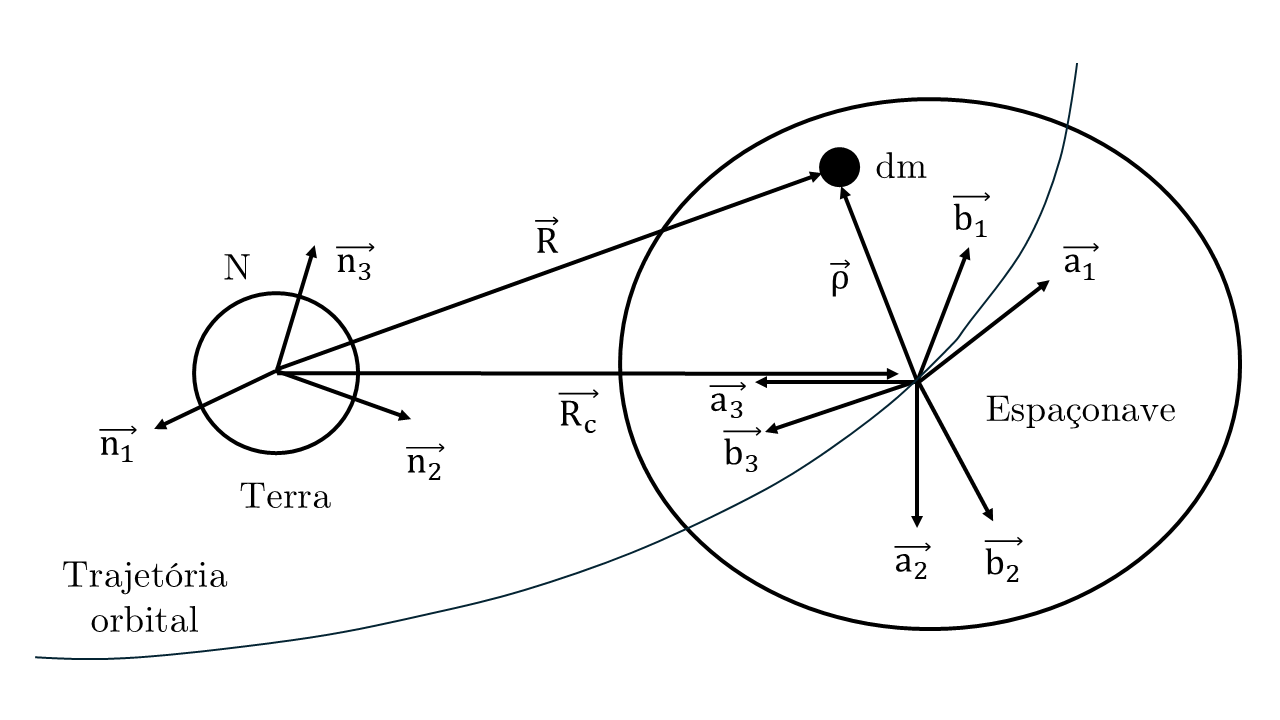
\includegraphics[width=1\textwidth]{4 Formulacao matematica/Imagens/Fig_6_8_Wie.png}
\caption{Geometria de um corpo rígido em órbita circular, com os referenciais inercial $N$, orbital $A$ e fixo ao corpo $B$. Adaptado de \cite{wie2008space}.}\label{fig_corporigido_wie}
\end{figure}

Na Figura~\ref{fig_corporigido_wie}, $\mu_\oplus$ representa o parâmetro gravitacional da Terra, $\vec{R}$ é o vetor posição do elemento de massa $dm$ em relação ao centro da Terra, $\vec{R}_c$ é o vetor posição do \gls{cdm} da espaçonave em relação ao centro da Terra, $\vec{\rho}$ é o vetor posição do elemento de massa $dm$ em relação ao \gls{cdm} da espaçonave, e $dm$ é um elemento infinitesimal de massa da espaçonave.
Assim, esses vetores se relacionam por:

\begin{equation}
\vec{R} = \vec{R}_c + \vec{\rho}.
\label{eq_relacao_R_Rc_rho}
\end{equation}

Além disso, $N$ denota o referencial inercial, $A=\{\vec{a}_1,\vec{a}_2,\vec{a}_3\}$ o referencial orbital e $B=\{\vec{b}_1,\vec{b}_2,\vec{b}_3\}$ o referencial fixo ao corpo da espaçonave.
Com base na geometria apresentada na Figura~\ref{fig_corporigido_wie}, a força gravitacional diferencial atuando sobre o elemento de massa $dm$ pode ser escrita como:

\begin{equation}
d\vec{f}
=
-\frac{\mu_\oplus \,\vec{R}}{\|\vec{R}\|^3}\,dm
=
-\frac{\mu_\oplus \,(\vec{R}_c+\vec{\rho})}{\|\vec{R}_c+\vec{\rho}\|^3}\,dm.
\label{eq_forca_gravitacional_dm}
\end{equation}

Em que os vetores $\vec{R}$, $\vec{R}_c$ e $\vec{\rho}$ são aqueles definidos na Figura~\ref{fig_corporigido_wie}.
A partir da força diferencial \(d\vec{f}\), o momento diferencial em torno do \gls{cdm} da espaçonave é dado por \(\vec{\rho}\times d\vec{f}\). Assim, o torque gravitacional resultante pode ser obtido pela integração sobre toda a distribuição de massa do corpo:

\begin{equation}
\vec{M}_{gg}
=
\int \vec{\rho}\times d\vec{f}.
\label{eq_torque_gg_integral}
\end{equation}

Essa expressão representa o torque de gradiente de gravidade, que surge devido à não uniformidade do campo gravitacional ao longo do corpo rígido em órbita.
De forma geral, a resultante dos momentos externos em torno do \gls{cdm} da espaçonave é relacionada à derivada temporal da quantidade de movimento angular por:

\begin{equation}
\vec{M}
=
\dot{\vec{H}}.
\label{eq_wie_M_Hdot}
\end{equation}

Em que $\vec{H}$ é a quantidade de movimento angular da espaçonave em torno do seu \gls{cdm}, e $\vec{M}$ representa o momento externo resultante.
Para uma espaçonave rígida em órbita circular, a integração do torque gravitacional ao longo da distribuição de massa conduz à expressão vetorial do torque de gradiente de gravidade, dada por:

\begin{equation}
\vec{M}_{gg}
=
3n^2\,\vec{a}_3 \times \left(\mathbf{I}\,\vec{a}_3\right).
\label{eq_torque_gradiente_gravidade}
\end{equation}

Em que $n$ é a velocidade angular orbital constante da órbita circular considerada, $\vec{a}_3$ é o versor do referencial orbital dirigido radialmente para a Terra e $\mathbf{I}$ é a matriz de inércia da espaçonave em torno do seu \gls{cdm}.
Seja $\mathbf{C}^{B/A}$ a matriz de rotação do referencial orbital $A$ para o referencial do corpo $B$. Nesse caso, o versor radial $\vec a_3$, expresso no referencial $B$, corresponde à terceira coluna de $\mathbf{C}^{B/A}$, isto é:

\begin{equation}
\vec a_3 =
\begin{bmatrix}
C_{13}\\
C_{23}\\
C_{33}
\end{bmatrix}.
\label{eq_a3_corpo}
\end{equation}

Em que $C_{13}$, $C_{23}$ e $C_{33}$ são os cossenos diretores associados à terceira coluna da matriz de rotação que descreve a orientação do referencial orbital $A$ em relação ao referencial do corpo $B$. Portanto, esses termos representam as componentes do versor radial $\vec a_3$ expressas no referencial $B$.
Por sua vez, a matriz de inércia é escrita como:

\begin{equation}
\mathbf{I}=
\begin{bmatrix}
I_{11} & I_{12} & I_{13}\\
I_{21} & I_{22} & I_{23}\\
I_{31} & I_{32} & I_{33}
\end{bmatrix}.
\label{eq_inercia_expandida_corpo}
\end{equation}

Em que $I_{ij}$, com $i,j=1,2,3$, representam os elementos da matriz de inércia da espaçonave expressa no referencial do corpo.
Para uma órbita circular de velocidade angular orbital constante $n$, a velocidade angular do referencial orbital $A$ em relação ao referencial inercial $N$ é dada por:

\begin{equation}
\vec{\omega}^{A/N} = -n\,\vec{a}_2.
\label{eq_omega_A_N}
\end{equation}

Em que $\vec{\omega}^{A/N}$ representa a velocidade angular do referencial orbital $A$ em relação ao referencial inercial $N$, $n$ é a velocidade angular orbital constante da órbita circular considerada e $\vec{a}_2$ é o versor associado ao eixo normal ao plano orbital no referencial $A$.
A velocidade angular da espaçonave em relação ao referencial inercial pode, então, ser escrita como:

\begin{equation}
\vec{\omega}^{B/N} = \vec{\omega}^{B/A} + \vec{\omega}^{A/N}.
\label{eq_omega_B_N_decomp}
\end{equation}

Em que $\vec{\omega}^{B/N}$ é a velocidade angular da espaçonave em relação ao referencial inercial $N$, $\vec{\omega}^{B/A}$ é a velocidade angular do corpo em relação ao referencial orbital e $\vec{\omega}^{A/N}$ é a velocidade angular do referencial orbital em relação ao referencial inercial.
A quantidade de movimento angular da espaçonave, expressa no referencial do corpo, é dada por:

\begin{equation}
\vec{H} = \mathbf{I}\,\vec{\omega}^{B/N}.
\label{eq_H_corpo_orbita}
\end{equation}

Em que $\mathbf{I}$ é a matriz de inércia da espaçonave em torno do seu \gls{cdm}, expressa no referencial $B$.
Aplicando o teorema do transporte para a derivada temporal da quantidade de movimento angular, obtém-se:

\begin{equation}
\left\{ \frac{d\vec{H}}{dt} \right\}_{N}
=
\left\{ \frac{d\vec{H}}{dt} \right\}_{B}
+
\vec{\omega}^{B/N}\times\vec{H}.
\label{eq_transporte_H_orbita}
\end{equation}

Como os eixos do referencial $B$ são assumidos alinhados aos eixos principais de inércia, a matriz $\mathbf{I}$ é constante nesse referencial e, portanto,

\begin{equation}
\left\{ \frac{d\vec{H}}{dt} \right\}_{B}
=
\mathbf{I}\,\dot{\vec{\omega}}^{B/N}.
\label{eq_dHdt_B_orbita}
\end{equation}

Em que $\dot{\vec{\omega}}^{B/N}$ representa a aceleração angular da espaçonave em relação ao referencial inercial, expressa no referencial do corpo.
Substituindo \eqref{eq_H_corpo_orbita} e \eqref{eq_dHdt_B_orbita} em \eqref{eq_transporte_H_orbita}, resulta:

\begin{equation}
\vec{M}
=
\mathbf{I}\,\dot{\vec{\omega}}^{B/N}
+
\vec{\omega}^{B/N}\times\left(\mathbf{I}\,\vec{\omega}^{B/N}\right).
\label{eq_euler_rotacional_wie}
\end{equation}


Para uma espaçonave rígida em órbita circular, o momento externo dominante associado ao acoplamento entre órbita e atitude é o torque de gradiente de gravidade $\vec{M}_{gg}$.
Substituindo \eqref{eq_torque_gradiente_gravidade} em \eqref{eq_euler_rotacional_wie}, obtém-se a equação de Euler para um corpo rígido em órbita circular:

\begin{equation}
\mathbf{I}\,\dot{\vec{\omega}}^{B/N}
+
\vec{\omega}^{B/N}\times\left(\mathbf{I}\,\vec{\omega}^{B/N}\right)
=
3n^2\,\vec{a}_3 \times \left(\mathbf{I}\,\vec{a}_3\right).
\label{eq_euler_corpo_rigido_orbita}
\end{equation}


A Equação~\eqref{eq_euler_corpo_rigido_orbita} corresponde ao modelo clássico de um corpo rígido em órbita circular. Sua forma matricial expandida pode ser escrita como:

\begin{equation} % atual equação 4.73
\begin{split}
&
\begin{bmatrix}
I_{11} & I_{12} & I_{13}\\
I_{21} & I_{22} & I_{23}\\
I_{31} & I_{32} & I_{33}
\end{bmatrix}
\begin{bmatrix}
\dot{\omega}_1\\
\dot{\omega}_2\\
\dot{\omega}_3
\end{bmatrix}
+
\begin{bmatrix}
0 & -\omega_3 & \omega_2\\
\omega_3 & 0 & -\omega_1\\
-\omega_2 & \omega_1 & 0
\end{bmatrix}
\begin{bmatrix}
I_{11} & I_{12} & I_{13}\\
I_{21} & I_{22} & I_{23}\\
I_{31} & I_{32} & I_{33}
\end{bmatrix}
\begin{bmatrix}
\omega_1\\
\omega_2\\
\omega_3
\end{bmatrix}
\\[1ex]
&=
3n^2
\begin{bmatrix}
0 & -C_{33} & C_{23}\\
C_{33} & 0 & -C_{13}\\
-C_{23} & C_{13} & 0
\end{bmatrix}
\begin{bmatrix}
I_{11} & I_{12} & I_{13}\\
I_{21} & I_{22} & I_{23}\\
I_{31} & I_{32} & I_{33}
\end{bmatrix}
\begin{bmatrix}
C_{13}\\
C_{23}\\
C_{33}
\end{bmatrix}.
\end{split}
\label{eq_euler_gg_expandida}
\end{equation}

Em que $\omega_1$, $\omega_2$ e $\omega_3$ representam as componentes de $\vec{\omega}^{B/N}$ no referencial do corpo, e $\dot{\omega}_1$, $\dot{\omega}_2$ e $\dot{\omega}_3$ são suas respectivas derivadas temporais.
No contexto desta dissertação, essa formulação é adotada como modelo-base da dinâmica de atitude de uma espaçonave rígida em órbita circular. Contudo, para a obtenção do modelo completo de atitude em órbita, essa dinâmica deve ser complementada pelas equações diferenciais da cinemática orbital, as quais serão apresentadas nas subseções seguintes.

Mesmo que o torque de gradiente de gravidade $\vec{M}_{gg}$, apresentado na Equação~\ref{eq_torque_gradiente_gravidade}, seja desconsiderado na modelagem dinâmica por ser tratado como uma perturbação de pequena magnitude, o efeito do movimento orbital não desaparece da formulação da atitude. Isso ocorre porque o referencial orbital \gls{lvlh} é não inercial e se move ao longo da órbita com velocidade angular orbital $n$.

Assim, no caso de um corpo rígido em órbita circular, a relação entre a velocidade angular da espaçonave e as taxas dos ângulos de Euler não coincide com aquela utilizada para um corpo rígido em solo ou em referencial inercial fixo. Em particular, a formulação cinemática deve incorporar explicitamente a contribuição da rotação orbital, conforme apresentado por \cite{wie2008space}. Dessa forma, a modelagem completa da atitude em órbita requer não apenas as equações dinâmicas de Euler, mas também as equações diferenciais da cinemática escritas de modo consistente com o referencial \gls{lvlh}. Nas subseções seguintes, essas relações cinemáticas serão apresentadas explicitamente, juntamente com as parametrizações da atitude empregadas neste trabalho.



%%%%%%%%%%%%%%%%%%%%%%%%%%%%%%%%%%%%%%%%%%%%%%%%%%%%%%
% %% Subseção 4.3.2
% \subsection{Matriz de inércia}
% \label{sec_matriz_inercia_variavel}

% No caso da espaçonave perseguidora, a distribuição de massa do sistema depende da configuração do \gls{mr}. Para estender a formulação anterior ao caso em que o \gls{mr} se movimenta, considera-se agora que a matriz de inércia da espaçonave robótica dependa da configuração interna do sistema.
% Nesta subseção, a atitude da espaçonave é representada por quatérnions unitários, denotados por $\vec{q}_B(t)$, enquanto a configuração do \gls{mr} é descrita pelo vetor de coordenadas articulares:

% \begin{equation}
% \vec{q}(t)=
% \begin{bmatrix}
% q_1(t) \\
% q_2(t) \\
% q_3(t)
% \end{bmatrix}.
% \label{eq_vetor_juntas_mr}
% \end{equation}

% Com a seguinte restrição:

% \begin{equation}
% \vec{q}_B^{\,T}(t)\,\vec{q}_B(t)=1.
% \label{eq_restricao_quaternion_unitario}
% \end{equation}

% Ressalta-se que os quatérnions são empregados nesta formulação como parâmetros de atitude, e não como coordenadas generalizadas independentes, uma vez que seus quatro elementos estão sujeitos à restrição de norma unitária \cite{wie2008space}.
% A matriz de inércia total em torno do \gls{cdm}, expressa no referencial do corpo $B$, é modelada por:

% \begin{equation}
% \mathbf{I}_B\big(\vec{q}(t)\big)
% =
% \mathbf{I}_{\text{perseg},B}
% +
% \mathbf{I}_{\text{manip},B}\big(\vec{q}(t)\big).
% \label{eq_inercia_total}
% \end{equation}

% O termo $\mathbf{I}_{\text{perseg},B}$ representa a matriz de inércia da espaçonave perseguidora, enquanto $\mathbf{I}_{\text{manip},B}\big(\vec{q}(t)\big)$ representa a contribuição do \gls{mr} durante o modo operacional, a qual depende da configuração das juntas e da orientação relativa dos elos em relação à espaçonave.
% Com base na formulação dinâmica de atitude em órbita apresentada anteriormente, a quantidade de movimento angular do sistema, expressa no referencial do corpo, é dada por:

% \begin{equation}
% \vec{H}_B(t)
% =
% \mathbf{I}_B\big(\vec{q}(t)\big)\,
% \vec{\omega}^{B/N}(t).
% \label{eq_H_def}
% \end{equation}

% A equação do momento angular mantém a forma geral:

% \begin{equation}
% \vec{M}
% =
% \left\{ \frac{d\vec{H}}{dt} \right\}_{N}.
% \label{eq_eq_momento_angular}
% \end{equation}

% Aplicando o teorema de transporte entre os referenciais $N$ e $B$, obtém-se \cite{wie2008space}:

% \begin{equation}
% \left\{ \frac{d\vec{H}_B}{dt} \right\}_{N}
% =
% \left\{ \frac{d\vec{H}_B}{dt} \right\}_{B}
% +
% \vec{\omega}^{B/N} \times \vec{H}_B.
% \label{eq_teorema_transporte_H}
% \end{equation}

% Substituindo \eqref{eq_H_def} em \eqref{eq_teorema_transporte_H} e utilizando \eqref{eq_eq_momento_angular}, obtém-se a equação do movimento rotacional para o sistema com matriz de inércia dependente da configuração:

% \begin{equation}
% \vec{M}
% =
% \mathbf{I}_B\big(\vec{q}(t)\big)\,
% \dot{\vec{\omega}}^{B/N}
% +
% \dot{\mathbf{I}}_B\big(\vec{q}(t)\big)\,
% \vec{\omega}^{B/N}
% +
% \vec{\omega}^{B/N} \times
% \left(
% \mathbf{I}_B\big(\vec{q}(t)\big)\,
% \vec{\omega}^{B/N}
% \right).
% \label{eq_euler_inercia_variavel}
% \end{equation}

% Na Equação~\eqref{eq_euler_inercia_variavel}, o termo
% $\vec{\omega}^{B/N} \times \left(\mathbf{I}_B(\vec{q}(t))\,\vec{\omega}^{B/N}\right)$
% representa o efeito giroscópico, enquanto o termo
% $\dot{\mathbf{I}}_B(\vec{q}(t))\,\vec{\omega}^{B/N}$
% representa a contribuição associada à variação temporal da matriz de inércia, decorrente da redistribuição interna de massa provocada pelo movimento do \gls{mr}.
% Para explicitar a dependência da configuração do sistema, a matriz de inércia $\mathbf{I}_B(\vec{q})$ pode ser escrita em termos de seus momentos e produtos de inércia, os quais variam conforme a posição das juntas:

% \begin{equation}
% \mathbf{I}_B\big(\vec{q}\big)
% =
% \begin{bmatrix}
% I_{xx}(\vec{q}) & -I_{xy}(\vec{q}) & -I_{xz}(\vec{q}) \\
% -I_{xy}(\vec{q}) & I_{yy}(\vec{q}) & -I_{yz}(\vec{q}) \\
% -I_{xz}(\vec{q}) & -I_{yz}(\vec{q}) & I_{zz}(\vec{q})
% \end{bmatrix}.
% \label{eq_matriz_inercia_expandida}
% \end{equation}

% Consequentemente, a taxa de variação temporal da matriz de inércia é obtida pela derivada total em relação ao tempo. Aplicando a regra da cadeia, tem-se:

% \begin{equation}
% \dot{\mathbf{I}}_B\big(\vec{q}, \dot{\vec{q}}\big)
% =
% \sum_{k=1}^{3}
% \frac{\partial \mathbf{I}_B(\vec{q})}{\partial q_k}\,\dot{q}_k.
% \label{eq_derivada_inercia_expandida}
% \end{equation}

% Em que $q_k$ é a $k$-ésima coordenada articular do manipulador e $\dot{q}_k$ é a respectiva velocidade da junta.